\documentclass[10pt,letterpaper]{article}

\usepackage{cogsci}
\usepackage{pslatex}
\usepackage{graphicx}
\usepackage{booktabs}
\usepackage{amsmath}
\usepackage{amssymb}
\usepackage{url}
\usepackage{caption}
\usepackage{subcaption}

\cogscifinalcopy

\graphicspath{{results/}}

\title{Where the Model Wanders and the Mind Converges: \\
A Distributional Comparison of Human and VARC Failures on ARC}

\author{{\large \bf Jing Yu} \\
  New York University \\
  \And
  {\large \bf Huijing Cong} \\
  New York University \\
  \And
  {\large \bf Elaine Zhou} \\
  New York University}

\date{}

\begin{document}
\maketitle

\begin{abstract}
The Abstraction and Reasoning Corpus (ARC) is one of the few benchmarks
where neural systems still perform worse than humans. Most prior work
only reports task-level accuracy, treating each task as pass or fail.
We argue this misses a more important difference in \emph{how} the two
agents fail. Using the official VARC ViT model's 510 multi-view
predictions per task and 946 participants from H-ARC, we treat each
side's responses as a distribution over answer grids and compare their
entropy, top-1 vote share, and number of distinct candidates. On the
111 tasks where humans succeed but VARC fails, humans settle on
$\approx 3.6$ distinct answers (top-1 share 74\%, entropy $0.80$);
VARC spreads across $\approx 264$ distinct grids (top-1 share 13\%,
entropy $4.72$). The correlation between human and VARC entropy is only
$r = 0.21$. We call this a \emph{failure-to-induce}: rather than picking
among a small hypothesis set as humans do, the model generates hundreds
of different grids, indicating that it often fails to induce a stable rule.

\textbf{Keywords:} ARC; visual reasoning; failure modes; entropy;
human-AI comparison
\end{abstract}

\section{Introduction}

The Abstraction and Reasoning Corpus~\cite{chollet2019measure} was
designed to be different from large supervised benchmarks: each task
gives only a few input--output examples and asks the solver to find a
transformation rule that works on a new input. Modern systems, including
the VARC family of vision transformers~\cite{varc}, have gotten much
closer to human performance, but a gap remains. The right question is
not how large this gap is, but \emph{what kind of failure causes it}.

Prior work mostly reports pass/fail accuracy on ARC, which hides what
is actually going wrong. The H-ARC dataset~\cite{harc} gives us the
human side: multiple participants attempt each task, and their final
grids are recorded. On the model side, VARC's inference already
provides something similar: each test input is processed through 510
augmented \emph{views}, and the final answer is a majority vote. The
distribution over these 510 outputs is not usually examined, but it
tells us what candidate answers the model is considering.

We use this parallel structure: both the $\sim 10$ human responses per
task and 510 VARC view predictions can be treated as distributions over
answer grids. We ask whether the \emph{shape} of these distributions
is different between humans and the model, especially on tasks where
humans succeed but VARC fails.

\paragraph{Contributions.}
\begin{itemize}
  \item We use VARC's existing 510-view predictions to measure model
        confidence at the task level with no additional computation.
  \item We define matching metrics for both human and model answer
        distributions and compare them across all 400 evaluation tasks.
  \item We find a clear difference: on tasks humans solve but VARC
        misses, humans focus on a few candidate answers while the model
        spreads across hundreds. We call this a
        \emph{failure-to-induce} signature.
\end{itemize}

\section{Methods}

\subsection{Data}

We use the 400-task ARC-AGI evaluation set. For the model side we use
VARC's official ARC-1\_ViT predictions, specifically the
\texttt{attempt\_0} folder (510 view-level predicted grids per task).
For the human side we use H-ARC's \texttt{summary\_data.csv} (7820
submissions from 946 participants). We only use evaluation tasks and
take each participant's last attempt as their final answer.
Table~\ref{tab:data} summarizes the data.

\begin{table}[t]
\centering
\begin{tabular}{lr}
\toprule
\textbf{Source} & \textbf{Count} \\
\midrule
ARC-1 evaluation tasks & 400 \\
VARC views per task (\texttt{attempt\_0}) & 510 \\
H-ARC participants & 946 \\
H-ARC answers (last attempt per task) & $\approx 10$ per task \\
\bottomrule
\end{tabular}
\caption{Data sources used in this study.}
\label{tab:data}
\end{table}

\subsection{Correctness scoring}

For VARC we follow the official plain-ViT scoring: keep the top-2
most-voted grids from 510 views; the task is correct if either matches
ground truth (pass@2). For humans we use \texttt{human\_accuracy}
(fraction of participants whose final answer is correct). To assign
tasks to quadrants in the Results section, we call the human
side ``correct'' when \texttt{human\_accuracy} $> 0.5$.

\subsection{Error typing}

For diagnostics we classify each predicted grid against ground truth:
\begin{itemize}
  \item \texttt{correct}: exact match.
  \item \texttt{wrong\_size}: row or column count differs.
  \item \texttt{close\_miss}: shape matches, cell accuracy $\geq 0.8$.
  \item \texttt{wrong\_content}: shape matches, cell accuracy $< 0.8$.
\end{itemize}
For VARC we use the top-1 voted grid, which is how the single most
likely output would normally be evaluated.

\subsection{Answer-distribution metrics}

Our main approach is to treat the 510 VARC views and $\sim 10$ human
answers as samples from answer distributions for each task. For each
task and each agent, we compute over the distribution of distinct grids
$\{g_i\}$ with vote counts $n_i$ (total $N$):
\begin{align*}
\text{top-1 share} &= \frac{\max_i n_i}{N},\\
\text{top-1/top-2 gap} &= \frac{n_{(1)} - n_{(2)}}{N},\\
H &= -\sum_i \frac{n_i}{N} \log \frac{n_i}{N}
   \quad\text{(Shannon entropy, in nats)},\\
n_{\mathrm{unique}} &= |\{g_i\}|.
\end{align*}
Both sides use the same units, so the metrics are directly comparable.

\subsection{Quadrant taxonomy}
\label{sec:quadrants}

We split the 400 tasks by joint correctness:
\begin{itemize}
  \item \texttt{both\_correct} ($n=173$),
  \item \texttt{human\_only} ($n=111$): human majority correct, VARC
        pass@2 wrong,
  \item \texttt{varc\_only} ($n=48$): VARC correct, human majority
        wrong,
  \item \texttt{both\_wrong} ($n=68$).
\end{itemize}
The \texttt{human\_only} group is our main focus: these are tasks that
humans can clearly solve, making VARC's failure most interesting.

\section{Results}
\label{sec:results}

\subsection{Aggregate accuracy and error type}

Across 400 tasks, mean human last-attempt accuracy is $64.1\%$ and
VARC pass@2 is $55.3\%$, matching the $55.63\%$ plain-ViT score
reported by Hu et al.~\cite{varc}. Table~\ref{tab:quadrants} shows
\texttt{human\_only} is the largest disagreement group: the model
misses 111 tasks that humans solve, more than twice the reverse.
Figure~\ref{fig:task_scatter} shows the per-task split.

\begin{table*}[t]
\centering\small
\begin{tabular}{lrrrr}
\toprule
 & both\_correct & human\_only & varc\_only & both\_wrong \\
\midrule
\# tasks & 173 & 111 & 48 & 68 \\
\bottomrule
\end{tabular}
\caption{Quadrant counts. \texttt{human\_only} is the largest
disagreement region.}
\label{tab:quadrants}
\end{table*}

\begin{figure}[t]
\centering
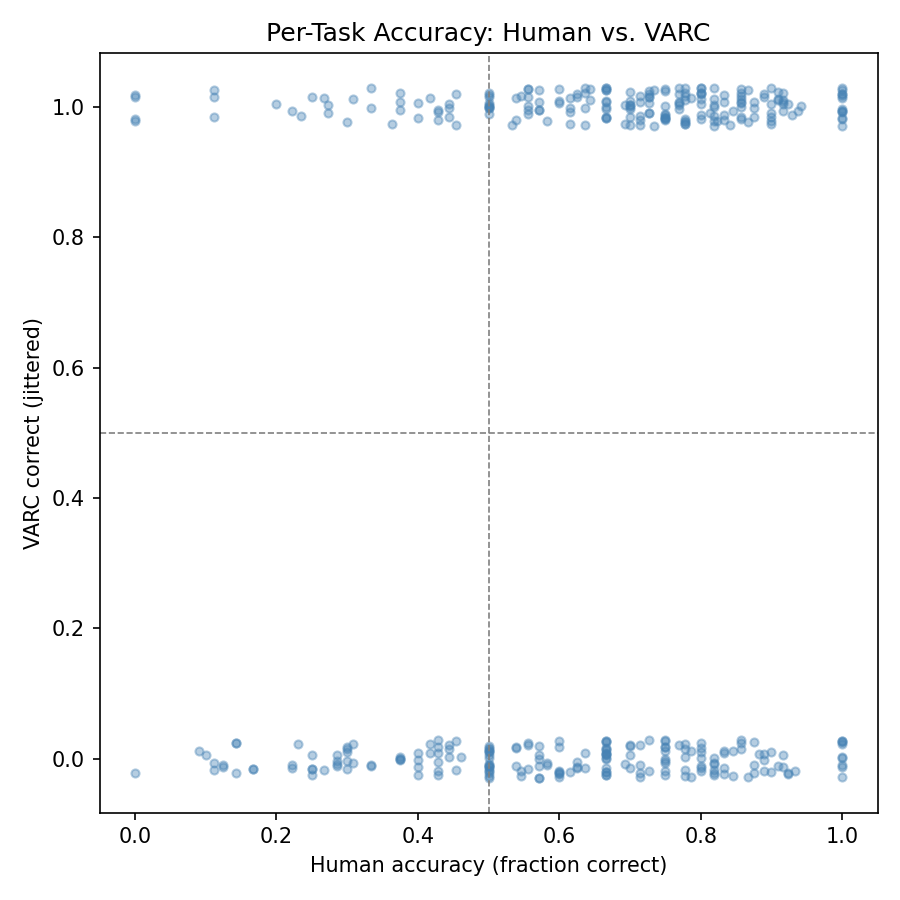
\includegraphics[width=\columnwidth]{task_accuracy_scatter.png}
\caption{Per-task accuracy. Each point is one ARC task; $y$-axis is
VARC binary correctness (jittered), $x$-axis is human accuracy. Points
cluster at the four quadrant corners.}
\label{fig:task_scatter}
\end{figure}

The two agents also fail with different error types.
Table~\ref{tab:varc_error_types} shows two thirds of VARC's wrong
answers are \texttt{close\_miss} --- the grid shape is right but a few
cells are wrong --- with the rest split between \texttt{wrong\_size}
and \texttt{wrong\_content}. Figure~\ref{fig:error_distribution} shows
the full distribution alongside the human side. Conditional on being
wrong, mean cell accuracy is $0.882$ for VARC and $0.739$ for humans
(Figure~\ref{fig:cell_acc_dist}): the model tends to get the structure
right but miss some cells, while humans more often get the content
completely wrong.

\begin{table}[t]
\centering
\begin{tabular}{lr}
\toprule
\textbf{VARC error type} (when wrong) & \textbf{Share} \\
\midrule
close\_miss     & $0.670$ \\
wrong\_size     & $0.179$ \\
wrong\_content  & $0.151$ \\
\bottomrule
\end{tabular}
\caption{VARC top-1 error distribution (wrong tasks only). Most
failures preserve grid shape and only miss a minority of cells.}
\label{tab:varc_error_types}
\end{table}

\begin{figure}[t]
\centering
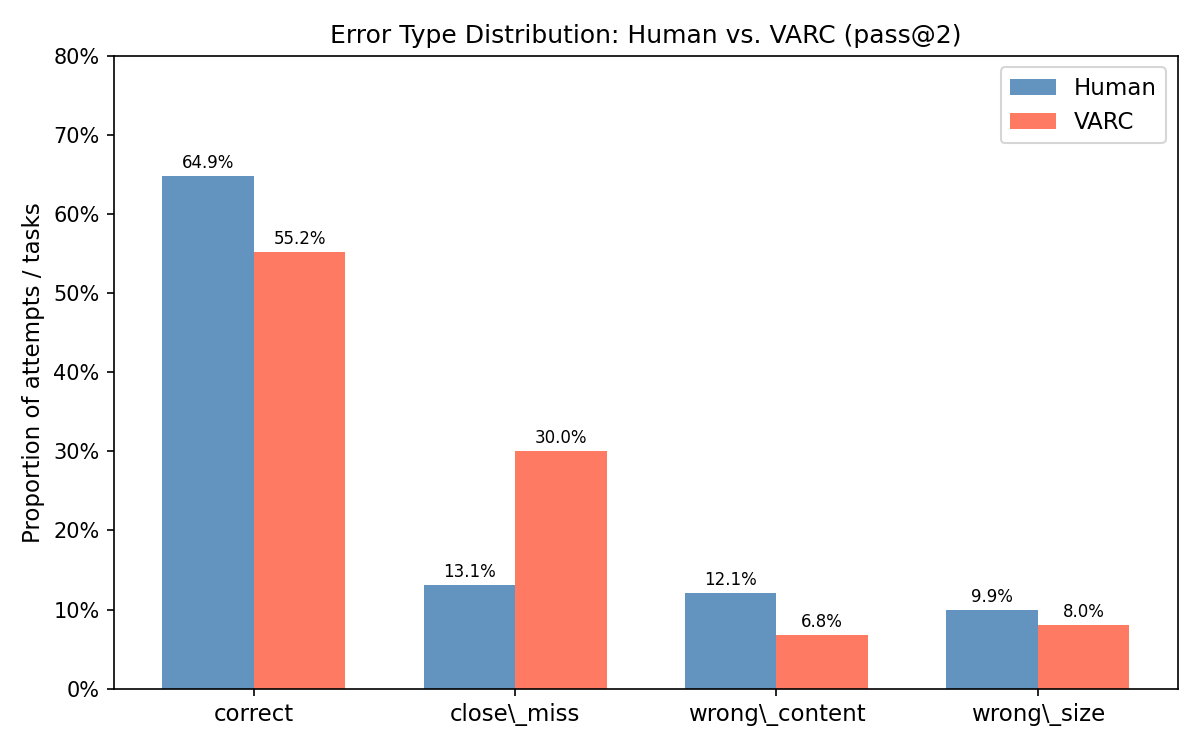
\includegraphics[width=\columnwidth]{error_distribution_pass2.png}
\caption{Error type distribution for VARC (pass@2) and humans across
all 400 tasks. VARC's correct bar uses pass@2 scoring (55.3\%); human
uses mean per-attempt accuracy (64.9\%). VARC clusters in
\texttt{close\_miss} while humans spread more evenly.}
\label{fig:error_distribution}
\end{figure}

\begin{figure}[t]
\centering
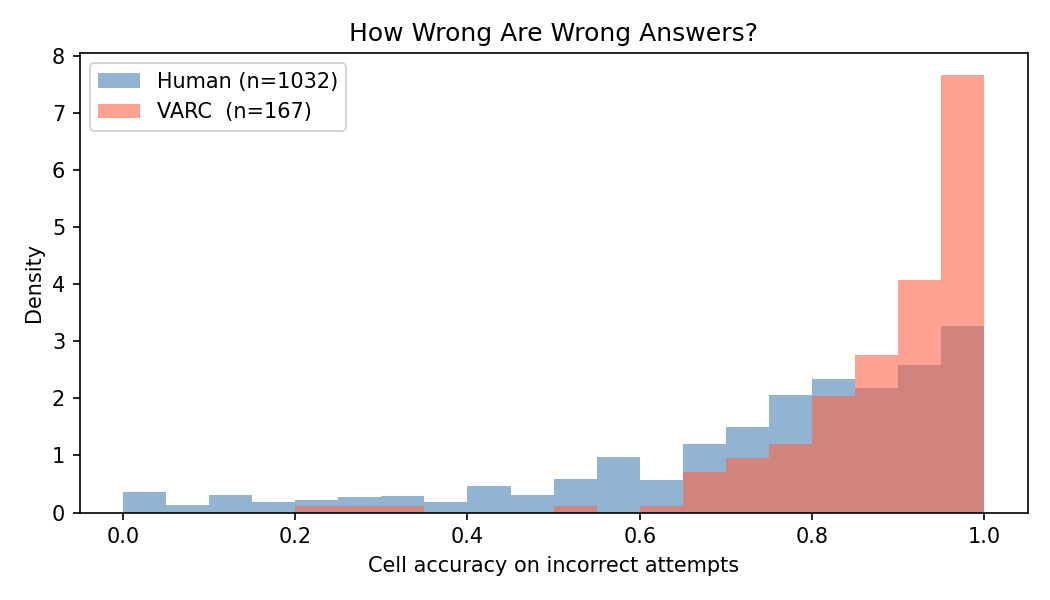
\includegraphics[width=\columnwidth]{cell_accuracy_dist.png}
\caption{Cell-level accuracy when wrong. VARC's mass concentrates near
$1.0$: most wrong predictions miss only a few cells. Human wrong
attempts spread across the range, with many low-accuracy submissions.}
\label{fig:cell_acc_dist}
\end{figure}

\subsection{VARC's view distribution tracks model confidence, not task
difficulty}
\label{sec:varc_view_dist}

Looking at VARC alone (Table~\ref{tab:varc_view}), there is a clear
pattern: when VARC is correct, its 510 views mostly agree on the same
answer; when VARC is wrong, the views spread across hundreds of
different outputs.

\begin{table*}[t]
\centering\small
\begin{tabular}{lrrrr}
\toprule
 & top-1 share & top-1/top-2 gap & vote entropy & \# unique grids \\
\midrule
both\_correct & 0.644 & 0.581 & 1.818 & 81.4 \\
varc\_only    & 0.618 & 0.557 & 1.997 & 91.6 \\
human\_only   & 0.125 & 0.071 & 4.724 & 263.7 \\
both\_wrong   & 0.110 & 0.065 & 4.914 & 280.9 \\
\bottomrule
\end{tabular}
\caption{VARC 510-view distribution metrics by quadrant. The top-1
share drops sharply on the two model-wrong rows, and those two rows
look nearly identical to each other.}
\label{tab:varc_view}
\end{table*}

Importantly, VARC's view spread looks almost the same for
\texttt{human\_only} and \texttt{both\_wrong}: entropy ($4.72$ vs
$4.91$) and unique-grid counts ($264$ vs $281$) are nearly identical.
The model is equally confused on tasks that humans can solve and tasks
that humans find difficult. This means the model's spread tells us whether
the model found an answer --- not whether the task is actually solvable.
Figure~\ref{fig:view_consistency} shows this: human accuracy varies a
lot within the high-entropy band, with \texttt{human\_only} (red) and
\texttt{both\_wrong} (gray) overlapping heavily.

\begin{figure*}[t]
\centering
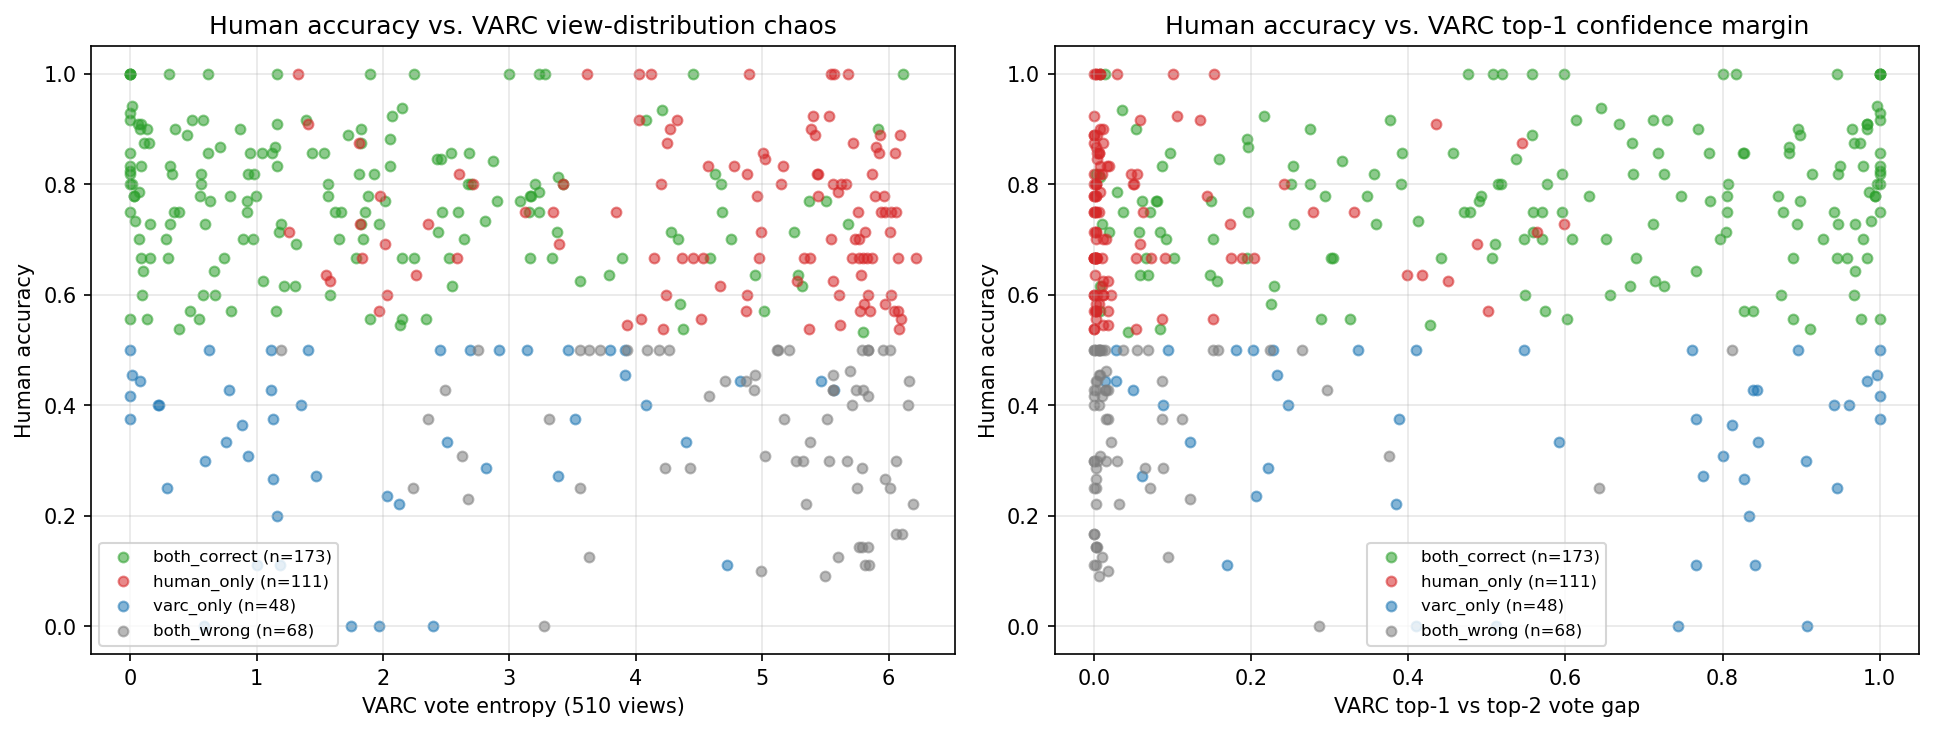
\includegraphics[width=\textwidth]{view_consistency_vs_human.png}
\caption{Human accuracy vs.\ VARC view-distribution entropy (left) and
top-1/top-2 margin (right). VARC's own confidence cleanly separates
VARC-correct (green/blue) from VARC-wrong (red/gray), but does not
separate \texttt{human\_only} (red) from \texttt{both\_wrong} (gray)
within the model-wrong band.}
\label{fig:view_consistency}
\end{figure*}

\subsection{Humans and VARC fail differently}
\label{sec:human_model}

Adding the human side (Table~\ref{tab:human_vs_varc},
Figure~\ref{fig:human_vs_varc}) makes the contrast clear.

\begin{table*}[t]
\centering\small
\begin{tabular}{lrrrr}
\toprule
 & VARC top-1 & VARC entropy & Human top-1 & Human entropy \\
\midrule
both\_correct & 0.644 & 1.818 & 0.774 & 0.716 \\
human\_only   & 0.125 & 4.724 & 0.741 & 0.800 \\
varc\_only    & 0.618 & 1.997 & 0.357 & 1.752 \\
both\_wrong   & 0.110 & 4.914 & 0.355 & 1.767 \\
\bottomrule
\end{tabular}
\caption{Top-1 share and entropy of VARC and human distributions per
quadrant. The \texttt{human\_only} row shows the key contrast: humans
concentrate (top-1 share 0.74, entropy 0.80) while VARC spreads
(top-1 share 0.13, entropy 4.72).}
\label{tab:human_vs_varc}
\end{table*}

\begin{figure*}[t]
\centering
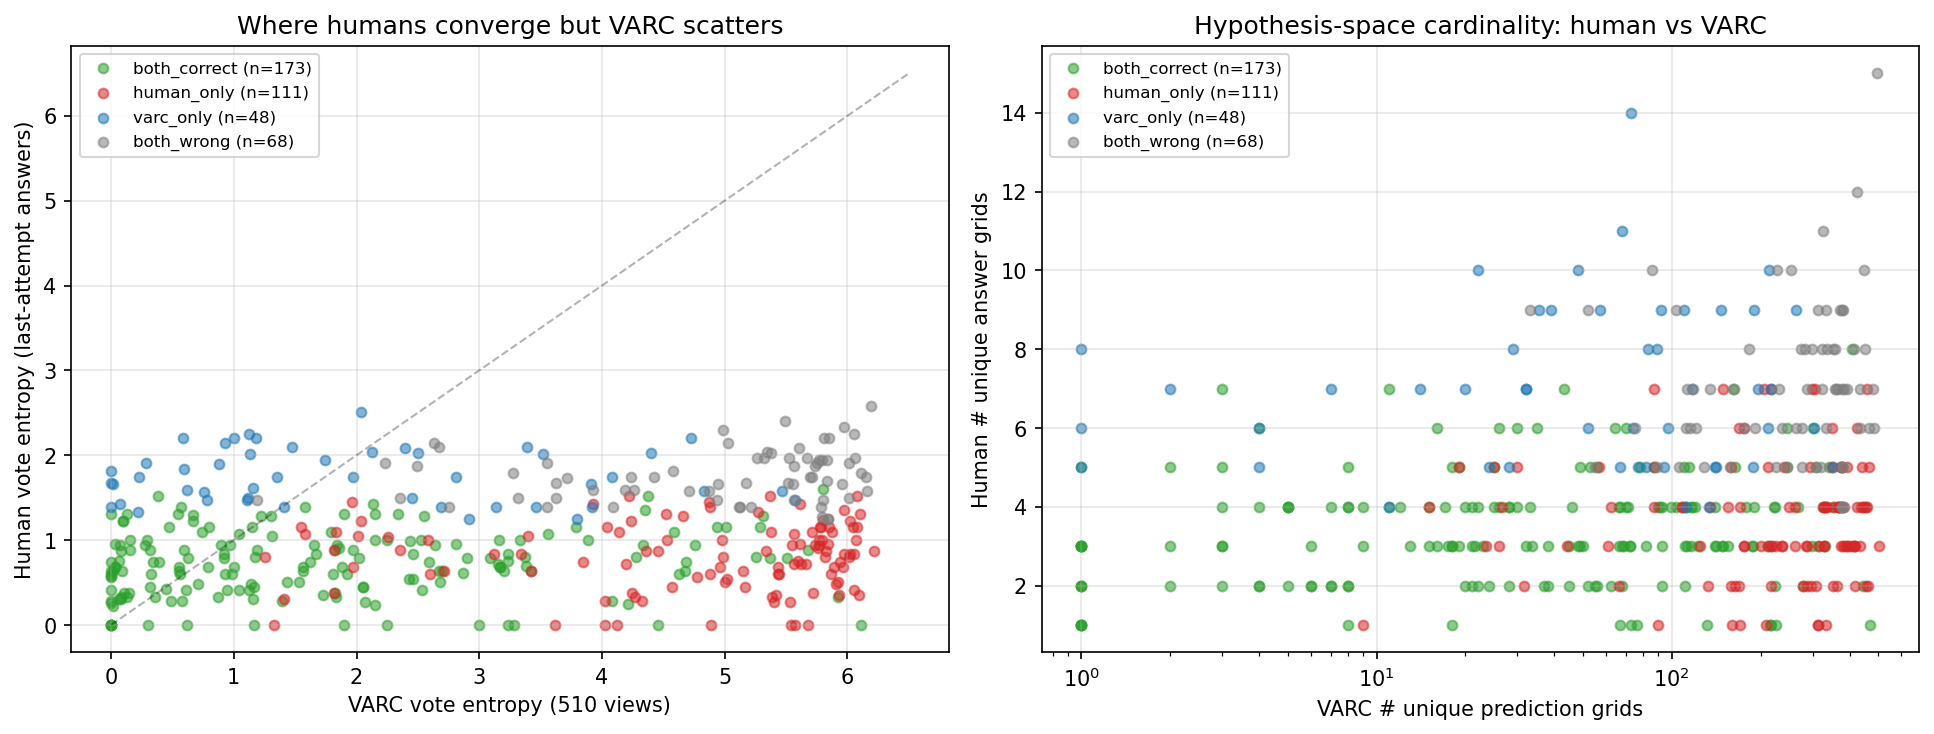
\includegraphics[width=\textwidth]{human_vs_varc_distribution.png}
\caption{VARC vs.\ human answer distributions per task. \emph{Left:}
entropy scatter; red points (\texttt{human\_only}) cluster far below
the $y=x$ line, showing humans converge while VARC scatters.
\emph{Right:} unique-grid counts (note log scale on VARC axis);
\texttt{human\_only} tasks place humans in the 2--5 grid regime and
VARC in the 100--500 grid regime.}
\label{fig:human_vs_varc}
\end{figure*}

Two results stand out. First, on \texttt{human\_only} tasks the
unique-grid count differs by nearly 100$\times$ ($\approx 3.6$
vs $\approx 264$). Humans don't just perform better; their responses
reflect a more consistent interpretation of the underlying rule,
leading to more similar error patterns. Second,
\texttt{both\_wrong} tasks show humans also spreading out (entropy
$1.77$, $\approx 7$ distinct grids) --- but still far less than VARC's
$\approx 281$ grids. Even when tasks are difficult for both humans and
the model, the human candidate set stays small; the model's does not.

The Pearson correlation between per-task VARC entropy and human entropy
is $r = 0.21$ ($p = 3.1 \times 10^{-5}$, $n = 400$), indicating a
weak association. This means tasks that are hard for humans and tasks
that are hard for VARC are mostly different tasks. In other words, the
two systems do not share a common notion of task difficulty, suggesting
a mismatch in their inductive biases.

The entropy gap on \texttt{human\_only} tasks is statistically robust.
A Mann-Whitney $U$ test comparing VARC vote entropy vs.\ human entropy
on \texttt{human\_only} tasks gives $U = 12291$, $p < 10^{-30}$
(one-sided), with a large effect size (Cohen's $d = 1.92$ relative to
\texttt{both\_correct}). Importantly, VARC entropy does \emph{not}
differ significantly between \texttt{human\_only} and
\texttt{both\_wrong} ($U = 3577$, $p = 0.56$), which further suggests
that the model's uncertainty is not aligned with human-defined task
difficulty.
Figure~\ref{fig:entropy_boxplot} shows the full per-quadrant
distributions.

\begin{figure*}[t]
\centering
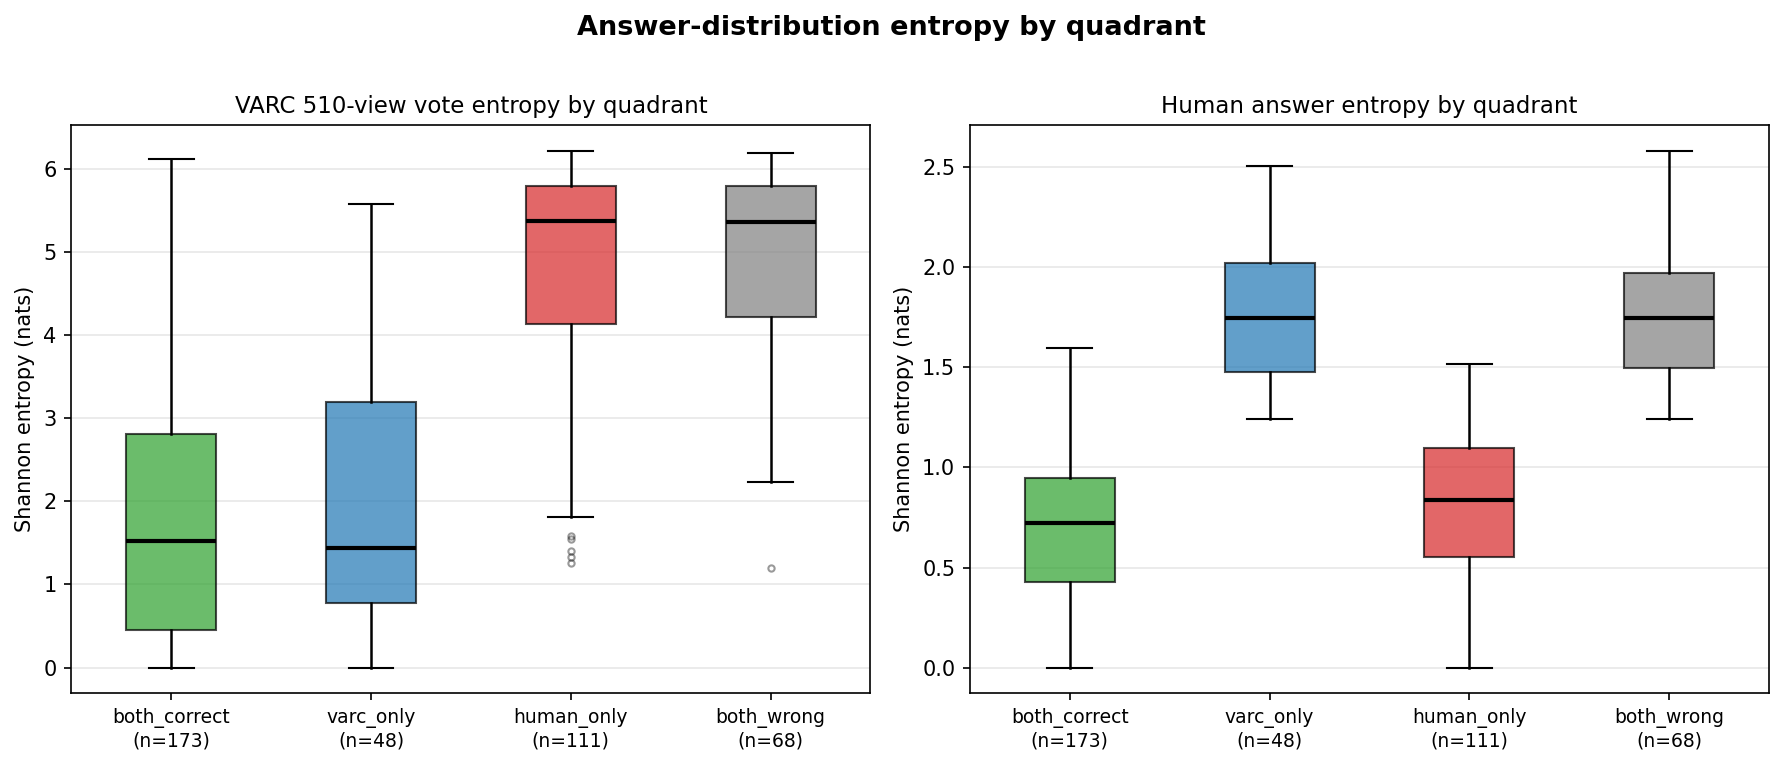
\includegraphics[width=\textwidth]{entropy_boxplot.png}
\caption{Per-quadrant entropy distributions. \emph{Left:} VARC vote
entropy. \emph{Right:} Human answer entropy. VARC cleanly separates
model-correct (low) from model-wrong (high). Human entropy is low for
both \texttt{both\_correct} and \texttt{human\_only}, and elevated for
\texttt{varc\_only} and \texttt{both\_wrong}. The overlap between
\texttt{human\_only} and \texttt{both\_wrong} on the left is
non-significant ($p = 0.56$).}
\label{fig:entropy_boxplot}
\end{figure*}

\subsection{Extreme cases: tasks with the largest entropy gap}
\label{sec:extreme}

To find the most striking individual tasks, we compute a per-task
\emph{entropy gap}
\[
  \Delta H_i \;=\; H_{\mathrm{VARC},i} - H_{\mathrm{Human},i}
\]
where both sides are measured in bits. We pool all four VARC
\texttt{attempt} folders (2\,040 predictions per task) to get a denser
sample; the human side is unchanged.
Figure~\ref{fig:entropy_gap_scatter} shows the entropy plane with the
ten largest-gap tasks circled.

\begin{figure}[t]
\centering
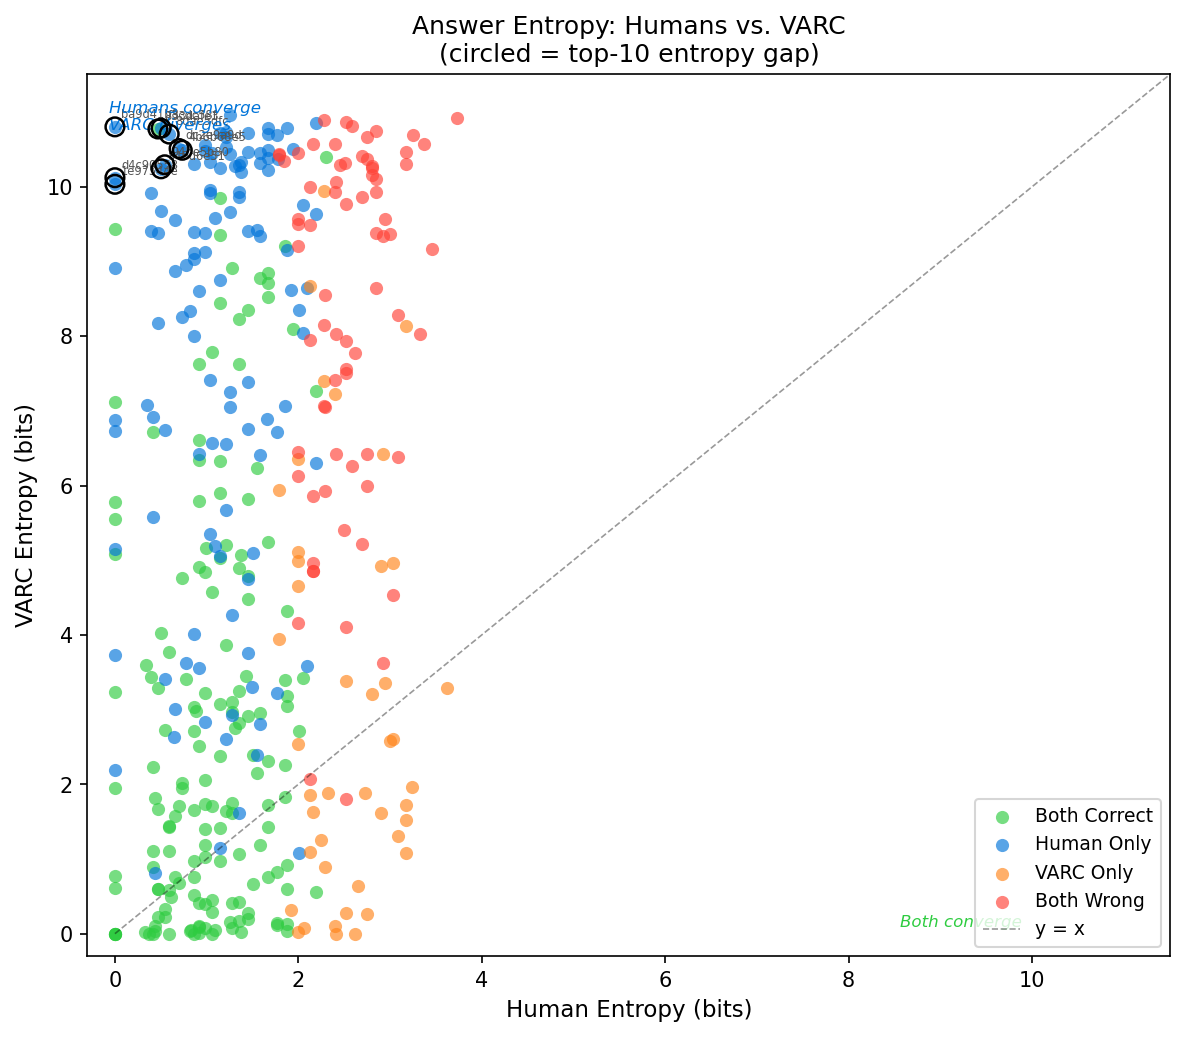
\includegraphics[width=\columnwidth]{entropy_gap_scatter.png}
\caption{Human vs.\ VARC entropy for all 400 tasks (2\,040 VARC
predictions). Tasks above the dashed diagonal have the model more
diffuse than humans; the ten circled points (upper-left corner) have
the largest $\Delta H$.}
\label{fig:entropy_gap_scatter}
\end{figure}

Table~\ref{tab:entropy_gap_top10} lists the top-10 tasks ranked by
$\Delta H$.

\begin{table*}[t]
\centering\small
\begin{tabular}{lrrrcc}
\toprule
\textbf{Task ID} & $H_{\mathrm{Human}}$ (bits) & $H_{\mathrm{VARC}}$ (bits) &
$\Delta H$ & Human acc. & VARC \\
\midrule
\texttt{ba9d41b8} & $\approx 0$ & $10.80$ & $10.80$ & $100\%$ & \texttimes \\
\texttt{d4c90558} & $\approx 0$ & $10.12$ & $10.12$ & $100\%$ & \texttimes \\
\texttt{1e97544e} & $\approx 0$ & $10.03$ & $10.03$ & $100\%$ & \texttimes \\
\texttt{833dafe3} & $0.47$      & $10.77$ & $10.31$ & $90\%$  & \checkmark \\
\texttt{f3cdc58f} & $0.50$      & $10.79$ & $10.28$ & $89\%$  & \texttimes \\
\texttt{8dae5dfc} & $0.59$      & $10.71$ & $10.11$ & $86\%$  & \texttimes \\
\texttt{dc2e9a9d} & $0.70$      & $10.51$ & $9.81$  & $87\%$  & \texttimes \\
\texttt{4b6b68e5} & $0.73$      & $10.49$ & $9.76$  & $86\%$  & \texttimes \\
\texttt{94be5b80} & $0.54$      & $10.30$ & $9.75$  & $88\%$  & \texttimes \\
\texttt{845d6e51} & $0.50$      & $10.24$ & $9.74$  & $89\%$  & \texttimes \\
\bottomrule
\end{tabular}
\caption{Top-10 tasks by entropy gap $\Delta H$ (bits, 2\,040 VARC
predictions). The three rows with $H_{\mathrm{Human}} \approx 0$ mark
tasks where every participant gave the same correct answer, while VARC
approaches the 11-bit theoretical maximum ($\log_2 2040 \approx 11.0$).}
\label{tab:entropy_gap_top10}
\end{table*}

The top three tasks are the most extreme. Human entropy is zero: every
participant gave the same correct answer (accuracy $= 100\%$). At the
same time, VARC entropy exceeds 10 bits: across 2,040 predictions the
model almost never gives the same answer twice.
Figures~\ref{fig:extreme_ba9d41b8}--\ref{fig:extreme_1e97544e} show
each task in full.

\begin{figure*}[t]
\centering
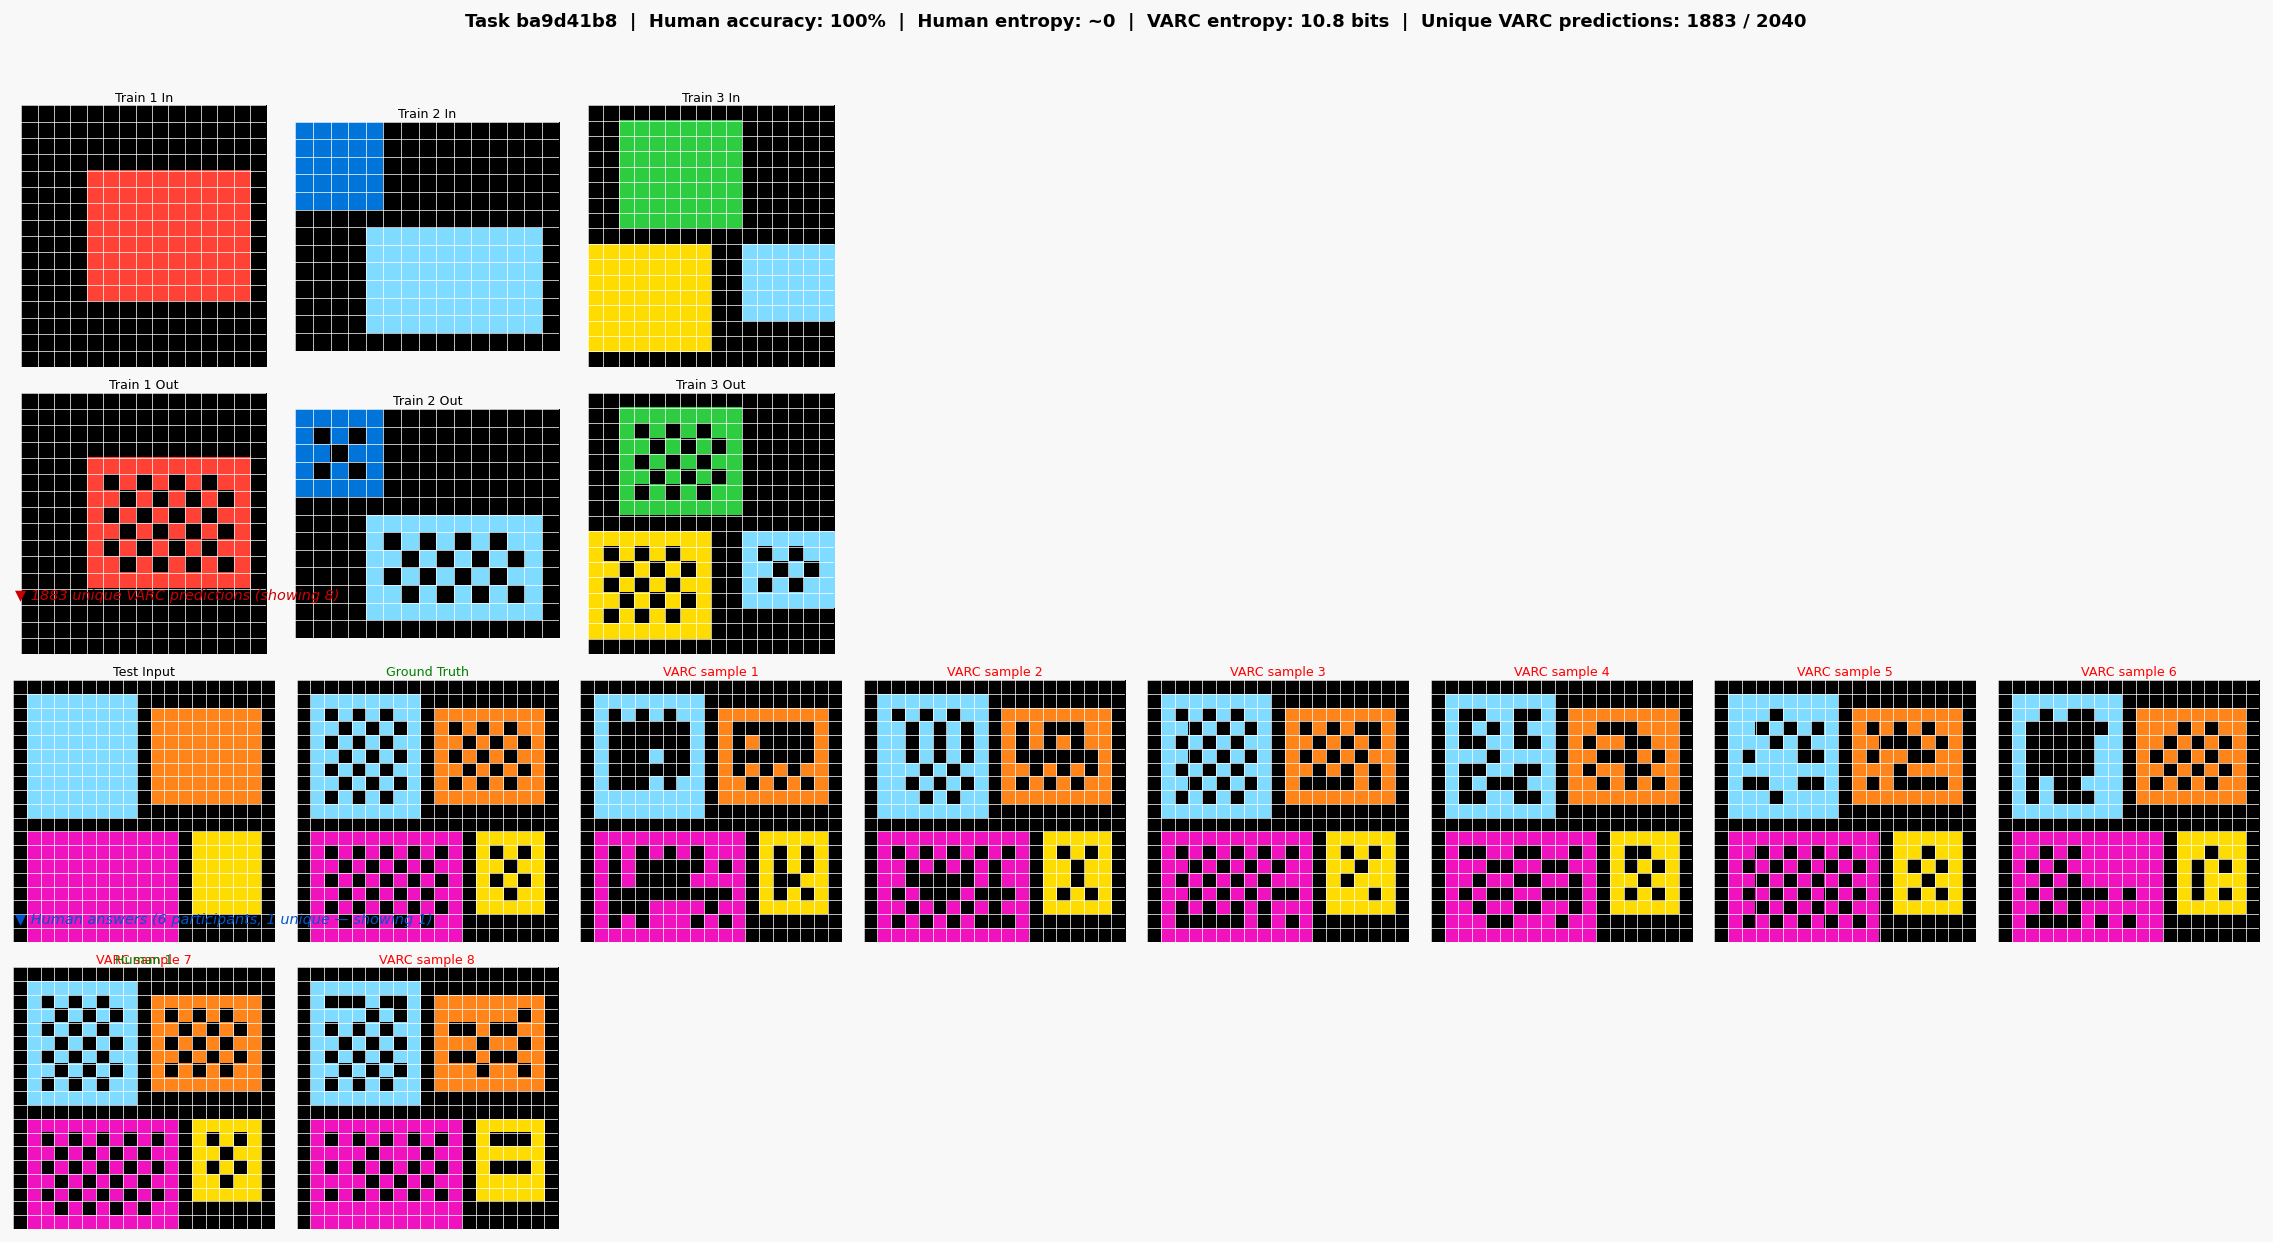
\includegraphics[width=\textwidth]{entropy_gap_top3_ba9d41b8.png}
\caption{Task \texttt{ba9d41b8} ($\Delta H = 10.80$ bits, the largest
gap in the dataset). \emph{Rows 1--2:} Training examples. \emph{Row 3:}
Test input, ground truth (green), and 8 sampled VARC predictions (red
--- nearly all unique among 2,040 views). \emph{Row 4:} Human final
answers, all correct.}
\label{fig:extreme_ba9d41b8}
\end{figure*}

\begin{figure*}[t]
\centering
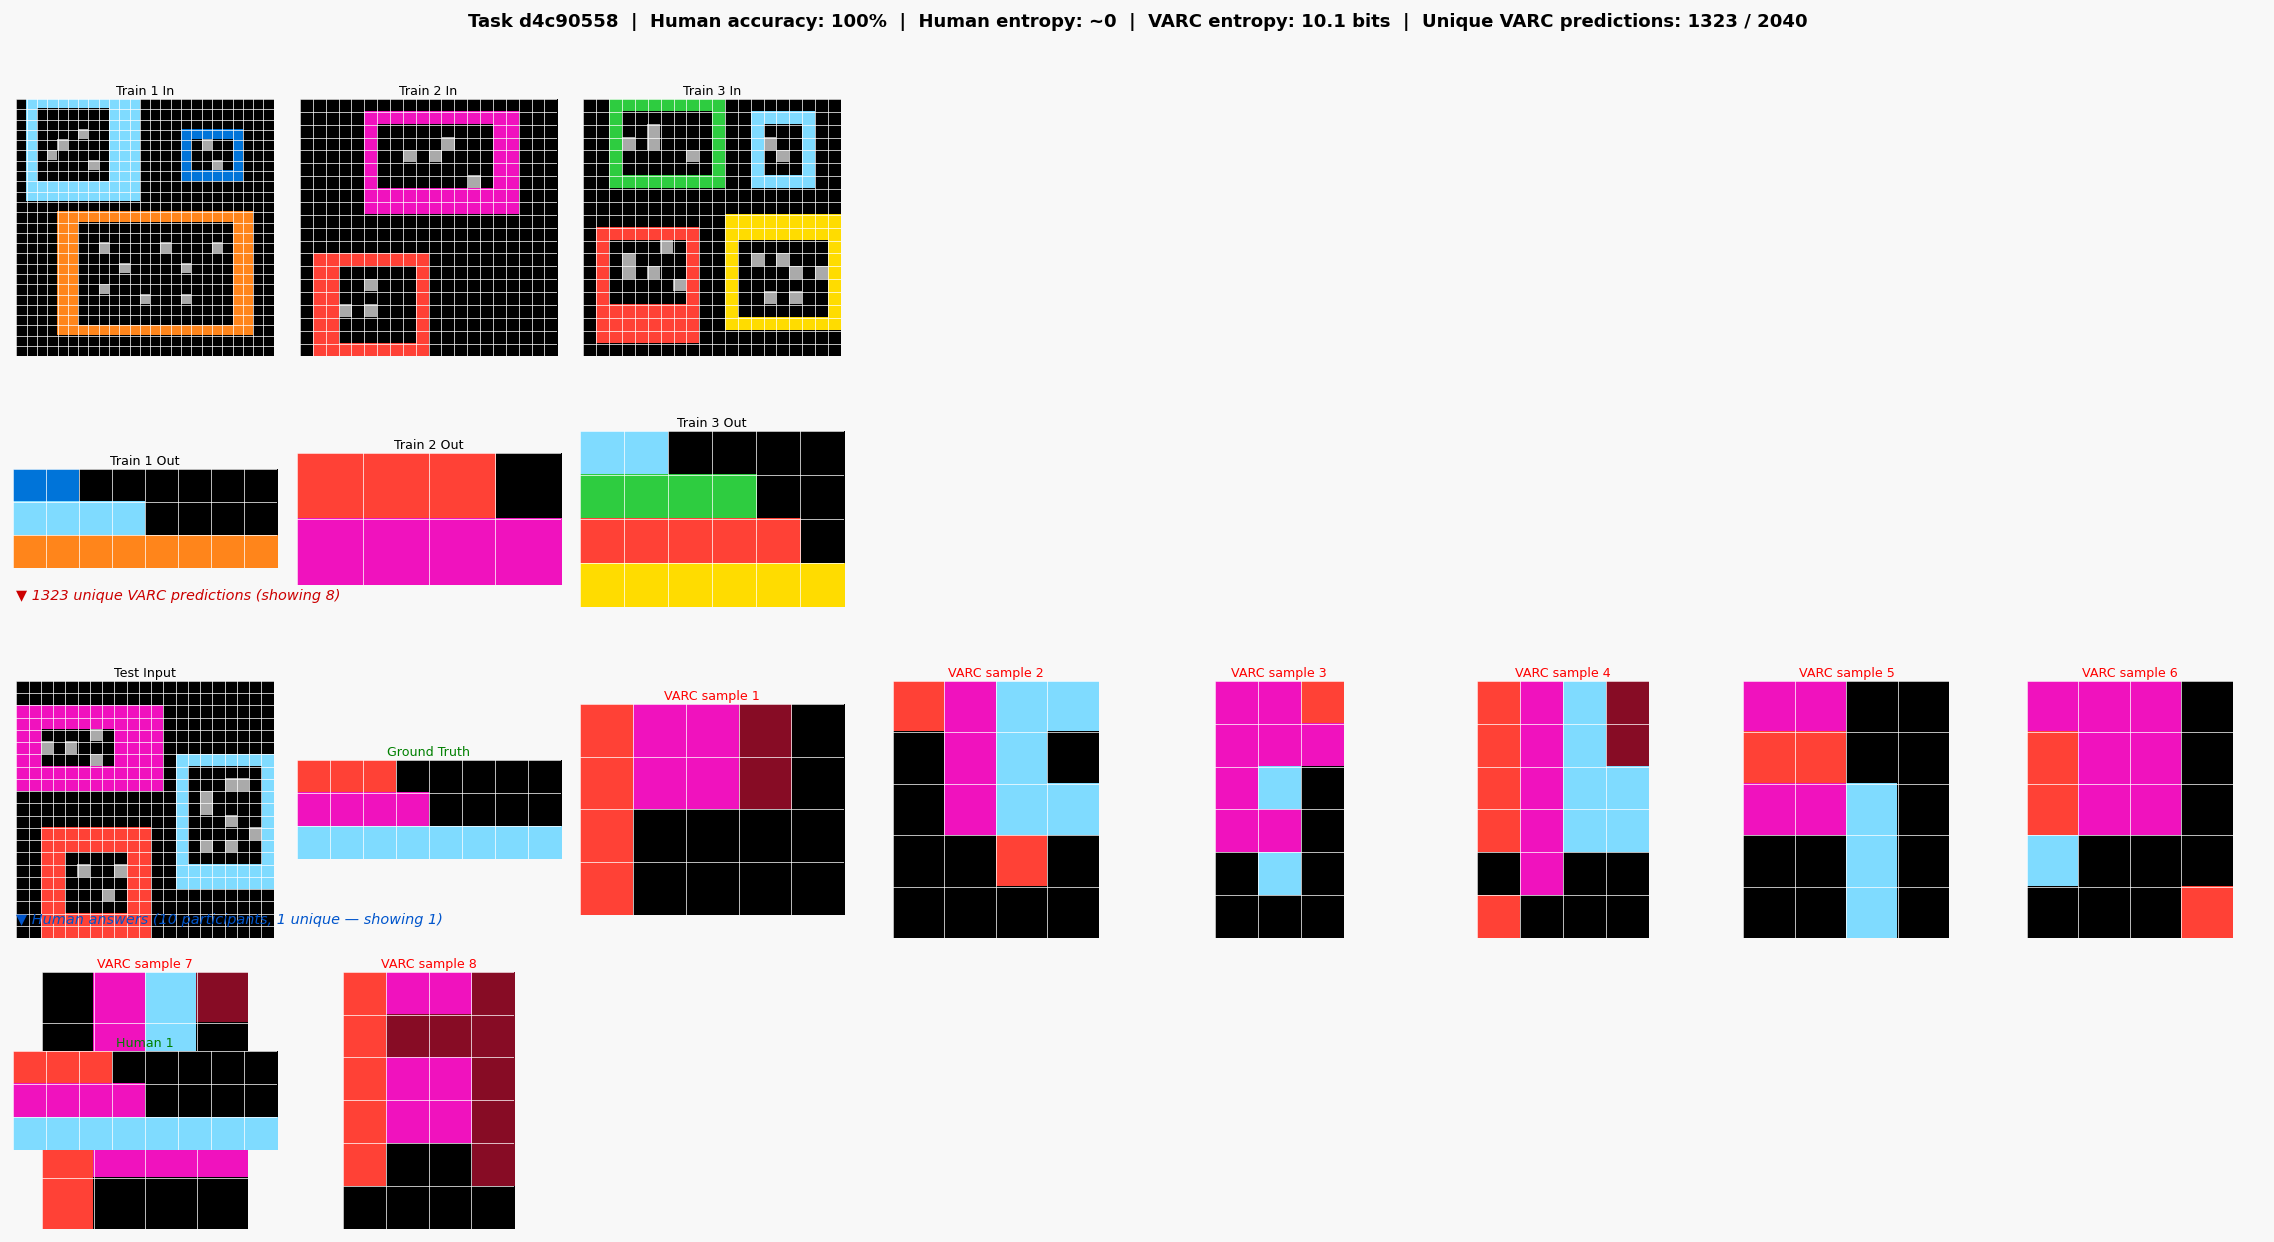
\includegraphics[width=\textwidth]{entropy_gap_top3_d4c90558.png}
\caption{Task \texttt{d4c90558} ($\Delta H = 10.12$ bits). Same layout
as Figure~\ref{fig:extreme_ba9d41b8}. Every human gives the correct
answer; VARC shows no convergence.}
\label{fig:extreme_d4c90558}
\end{figure*}

\begin{figure*}[t]
\centering
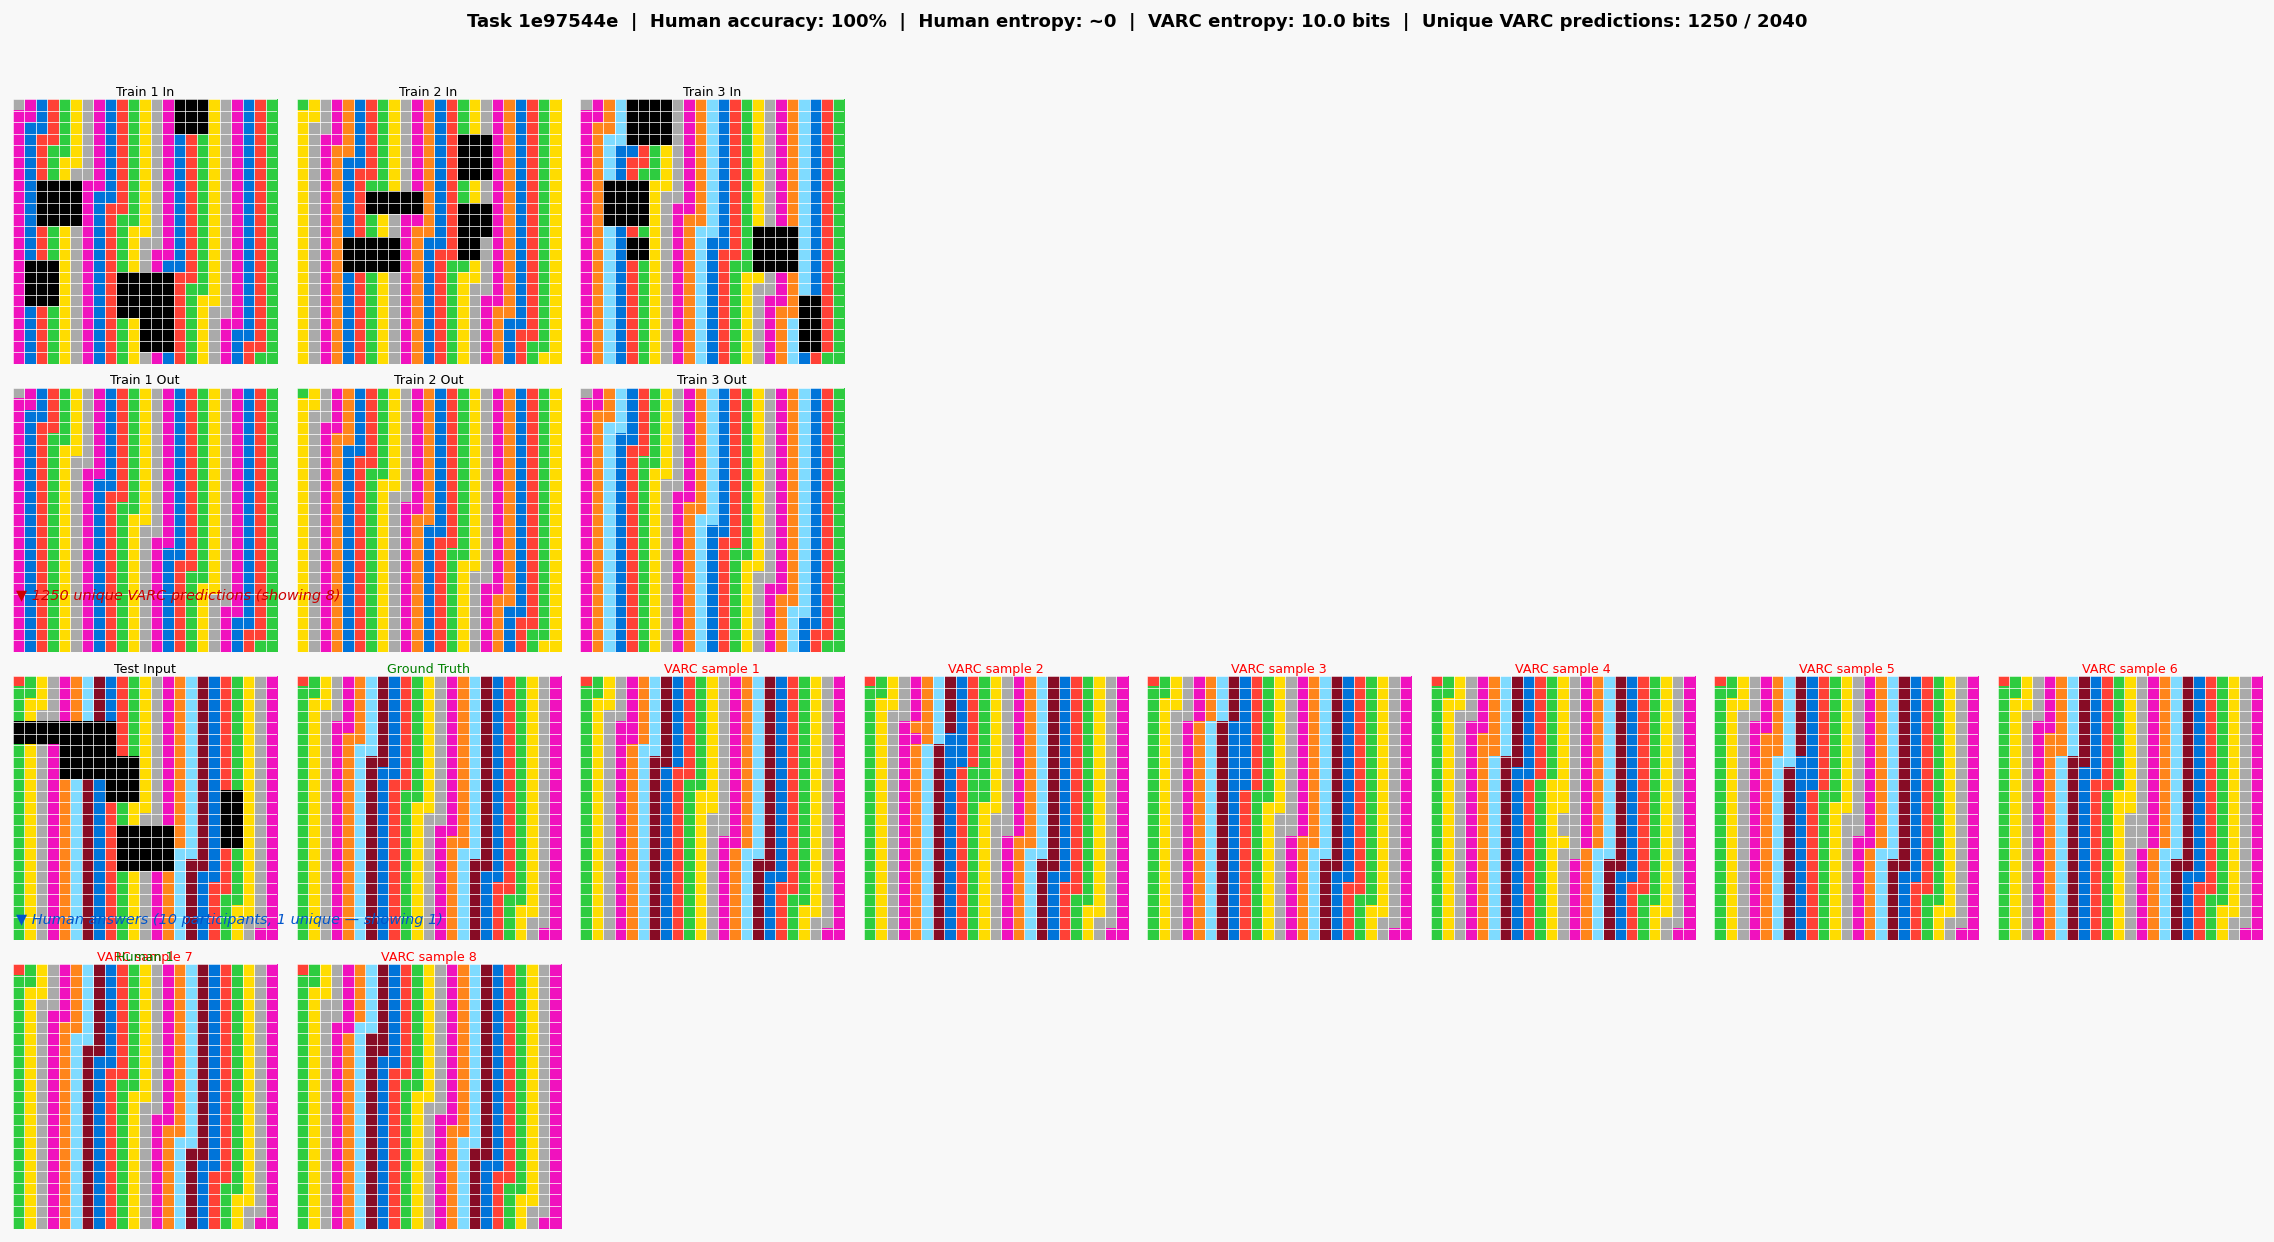
\includegraphics[width=\textwidth]{entropy_gap_top3_1e97544e.png}
\caption{Task \texttt{1e97544e} ($\Delta H = 10.03$ bits). Same layout
as Figure~\ref{fig:extreme_ba9d41b8}.}
\label{fig:extreme_1e97544e}
\end{figure*}

These three cases show that the high entropy in the
\texttt{human\_only} group is not just an averaging effect. At the
individual task level, the failure-to-induce pattern is as extreme as
it can get: every human gets it right, but VARC spreads across nearly
every possible answer.

\subsection{Qualitative illustration}

Figure~\ref{fig:qualitative} shows a specific \texttt{human\_only}
task (\texttt{b457fec5}) that clearly illustrates the failure-to-induce
pattern. The training examples reveal a simple rule: a grey diagonal
stripe gets recoloured using small marker squares placed along it.
Among the 12 participants who attempted the task, all final answers fell
into at most 3 distinct grids (entropy $0.87$), with the most common
answer matching ground truth exactly. VARC's 510 views, by contrast,
spread across \textbf{504 distinct grids} (entropy $6.22$) --- nearly a
uniform distribution over the output space. The model's top-1 prediction
has roughly the right structure but applies colours inconsistently, and
no single prediction gets more than a tiny fraction of the vote. This
is not a model that ``almost gets it'': it is a model that never settled
on any stable hypothesis about what the rule is.

\begin{figure*}[t]
\centering
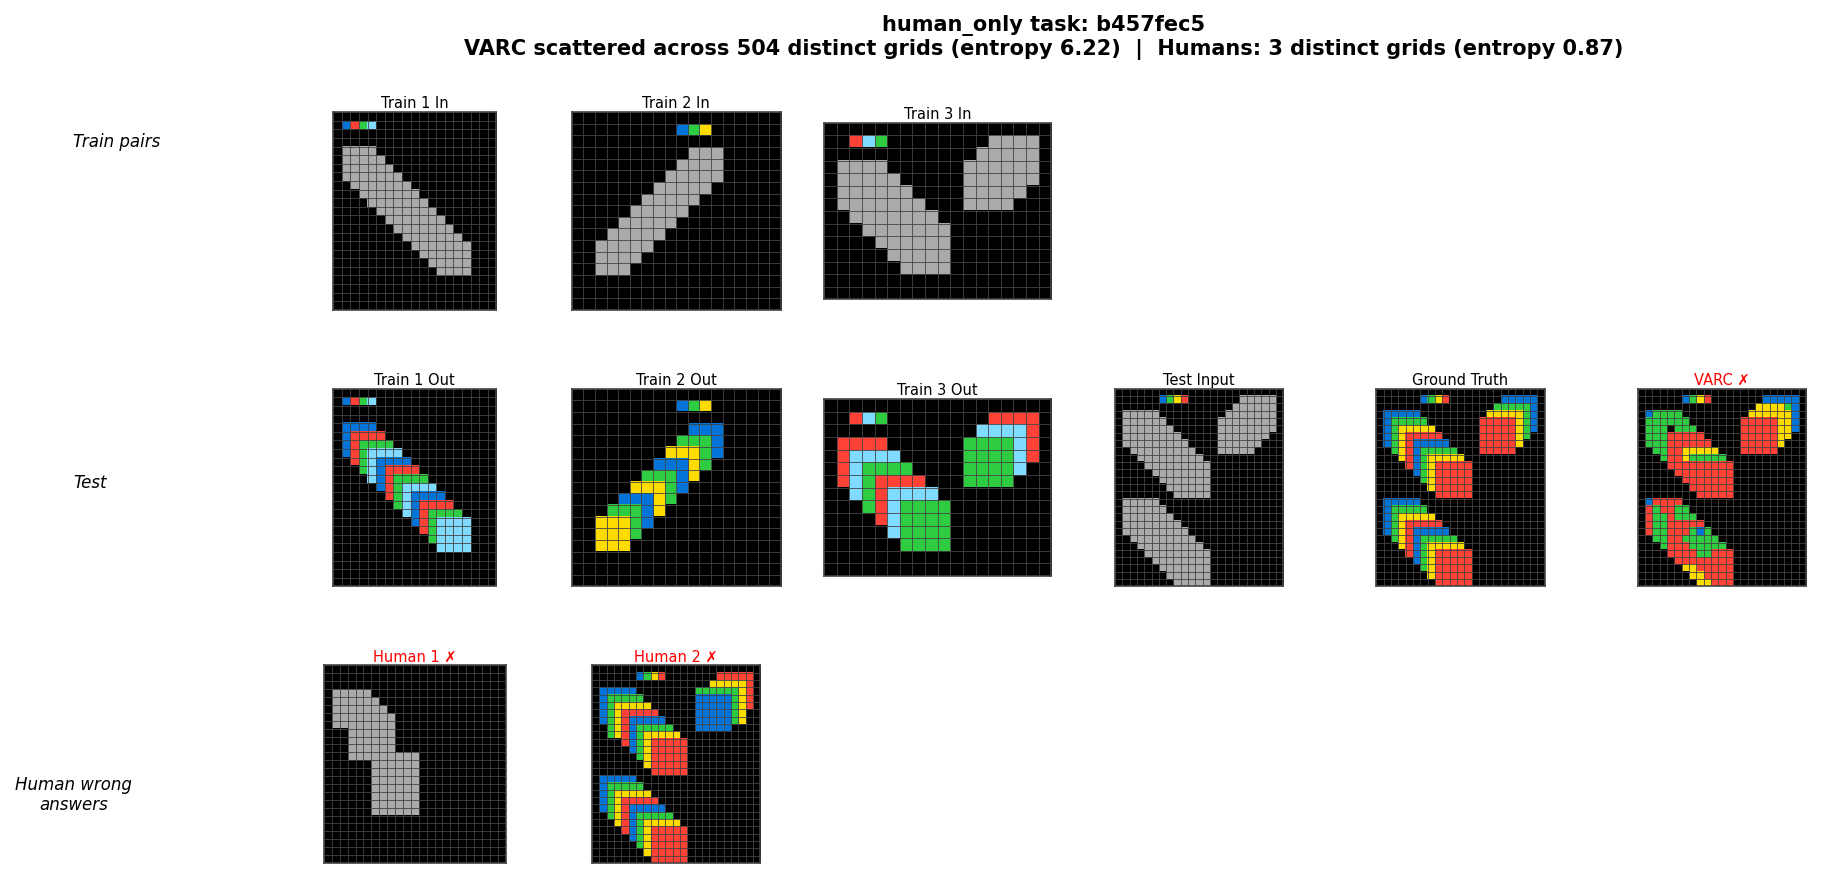
\includegraphics[width=\textwidth]{qualitative_example.png}
\caption{A \texttt{human\_only} task (\texttt{b457fec5}).
\emph{Row 1:} Training inputs.
\emph{Row 2:} Training outputs, test input, ground truth, and VARC's
top-1 prediction (red label).
\emph{Row 3:} Representative wrong human answers.
Humans produce only 3 distinct final answers (entropy $0.87$); VARC
spreads across 504 distinct grids (entropy $6.22$).}
\label{fig:qualitative}
\end{figure*}

\section{Discussion and Conclusion}

\subsection{Failure-to-induce}

Our main finding is that the two agents are not failing in the same way.
Human errors --- both on \texttt{human\_only} (when participants
disagree) and on \texttt{both\_wrong} (when nobody gets it right) ---
stay within a small set of candidate answers, typically reflecting
plausible but competing transformation rules. In contrast, VARC's
outputs are highly dispersed, spanning hundreds of distinct grids per
task. It shows that the model lacks a consistent understanding of the
underlying transformation.

We call this signature \emph{failure-to-induce}. VARC's multi-view
procedure samples augmented presentations of the same input. A model
that had found a transformation rule should give roughly the same answer
across views --- the rule should be view-invariant. The fact that 510
views produce hundreds of different outputs on VARC's failure tasks
suggests no such rule was ever found.

\subsection{Why VARC's own confidence isn't enough}

A natural idea is to use VARC's own view-level spread as a confidence
signal: low entropy means ``model is confident,'' high entropy means
``model is confused.'' The view-level distribution analysis below shows this
signal is real but limited: it cleanly separates VARC-correct from
VARC-wrong, but cannot separate \texttt{human\_only} from
\texttt{both\_wrong}. The model is equally confused on tasks that
humans can solve and on tasks that humans find difficult. Without the
human-side baseline, self-reported model confidence does not identify
the most important failures.

\subsection{Limitations}

Our approach is passive: we use VARC's existing 510 views rather than
designing controlled input edits (color swaps, rotation, etc.). This
means we can describe the shape of failure but cannot identify its
causal source. We also use only the plain-ViT \texttt{attempt\_0}
configuration; the full ensemble may exhibit slightly different
behavior. Human entropy estimates are limited by the $\approx 10$
participants per task.

\subsection{Future work}

A natural next step is to apply mechanistic causal probing to VARC.
By combining linear probes to locate relevant layers and then
intervening on those representations, we can identify where the model
starts to behave in a human-like way and where it breaks down.
This could help explain the mismatch between human and model failure
modes.

\subsection{Conclusion}

Our results reveal a qualitative difference beyond accuracy. Human
errors are structured and convergent: responses cluster around a small
set of plausible answers, reflecting a shared hypothesis space and
common inductive biases. In contrast, VARC's errors are highly
dispersed, spreading across hundreds of grids with little consensus.
This divergence does not track task difficulty, but instead suggests
that the model fails to form a coherent hypothesis. Bridging this gap
may require architectures that explicitly represent and search over
structured transformation rules.

\begin{thebibliography}{9}

\bibitem{chollet2019measure}
F.~Chollet,
\newblock On the Measure of Intelligence,
\newblock arXiv:1911.01547, 2019.
\newblock \url{https://arxiv.org/abs/1911.01547}.

\bibitem{varc}
K.~Hu, A.~Cy, L.~Qiu, X.~D.~Ding, R.~Wang, Y.~E.~Zhu, J.~Andreas, and K.~He,
\newblock {ARC} Is a Vision Problem!,
\newblock arXiv:2511.14761, 2025.
\newblock \url{https://arxiv.org/abs/2511.14761}.

\bibitem{harc}
S.~LeGris, W.~Vong, B.~M.~Lake, and T.~M.~Gureckis,
\newblock H-ARC,
\newblock OSF, 2025.
\newblock \url{https://doi.org/10.17605/OSF.IO/BH8YQ}.

\end{thebibliography}

\end{document}
